\chapter{Besoins nécessitant l'utilisation de services web}

\section{Définitions}

\begin{description}
\item[uid:] identifiant unique numérique au sein d'une base de données d'un échan\-tillon ;
\item[guid:] identifiant de type UUID\footnote{Les codes de type GUID ou UUID sont générés à partir de fonctions aléatoires ou cryptographiques, et garantissent qu'ils sont uniques quelle que soit la base de données qui les ont générés. Ainsi, il n'est pas possible d'obtenir deux codes identiques pour deux échantillons différents, ce qui permet de les identifier de manière sûre, comme pourrait le faire l'ADN pour des êtres humains.}, qui garantit de manière certaine l'identification d'un échantillon ;
\item [identifier :] identifiant \og métier \fg{} d'un échantillon;
\item [données \og métier \fg{} :] données permettant de caractériser un échantillon selon les critères nécessaires à son exploitation : contexte spécifique d'acquisition, taxon, données physico-chimiques ou biologiques, etc.
\item [instance, serveur, base de données, application :] implémentation d'une solution de gestion d'échantillons capable soit de fournir des services web, soit d'interroger des services web pour récupérer des informations.
\end{description}
\section{Présentation}

La gestion des échantillons de laboratoire (ou autres) est réalisée par divers logiciels, chacun s'appuyant sur une base de données différente. Dans un contexte d'échange des informations entre laboratoires, il est apparu nécessaire de proposer une méthode d'interrogation des différentes bases de données, pour connaître ce qui est disponible dans d'autres collections.

Deux cas d'utilisation ont ainsi pu être mis en évidence :
\begin{itemize}
\item l'interrogation d'une base distante, pour savoir si des échantillons sont disponibles ;
\item l'import d'informations provenant d'une autre base de données, pour ré\-pondre à deux cas de figure différents :
\begin{itemize}
\item le prêt d'un échantillon à un autre laboratoire, sans être obligé de ressaisir toutes les métadonnées associées ;
\item l'importation de données saisies sur le terrain en mode déconnecté dans une base de données centrale.
\end{itemize}
\end{itemize}

La technologie retenue est celle des services web, avec une gestion des habilitations s'inspirant du protocole OAuth v2.

\subsection{Technique employée}

Les services web sont basés sur des requêtes HTTP, et échangent les données selon des formats définis. Dans la version actuelle des services web, seul le format Json est implémenté pour l'échange des informations.

\subsection{Forme des URL}
Les URL sont conçues, dans le cadre des services web, sous la forme d'URL conviviales, par exemple : \url{https://collec/sw/v1/sample/4} pour récupérer l'échan\-tillon numéro 4.

\section{Définition des cas d'utilisation couverts par les services web}

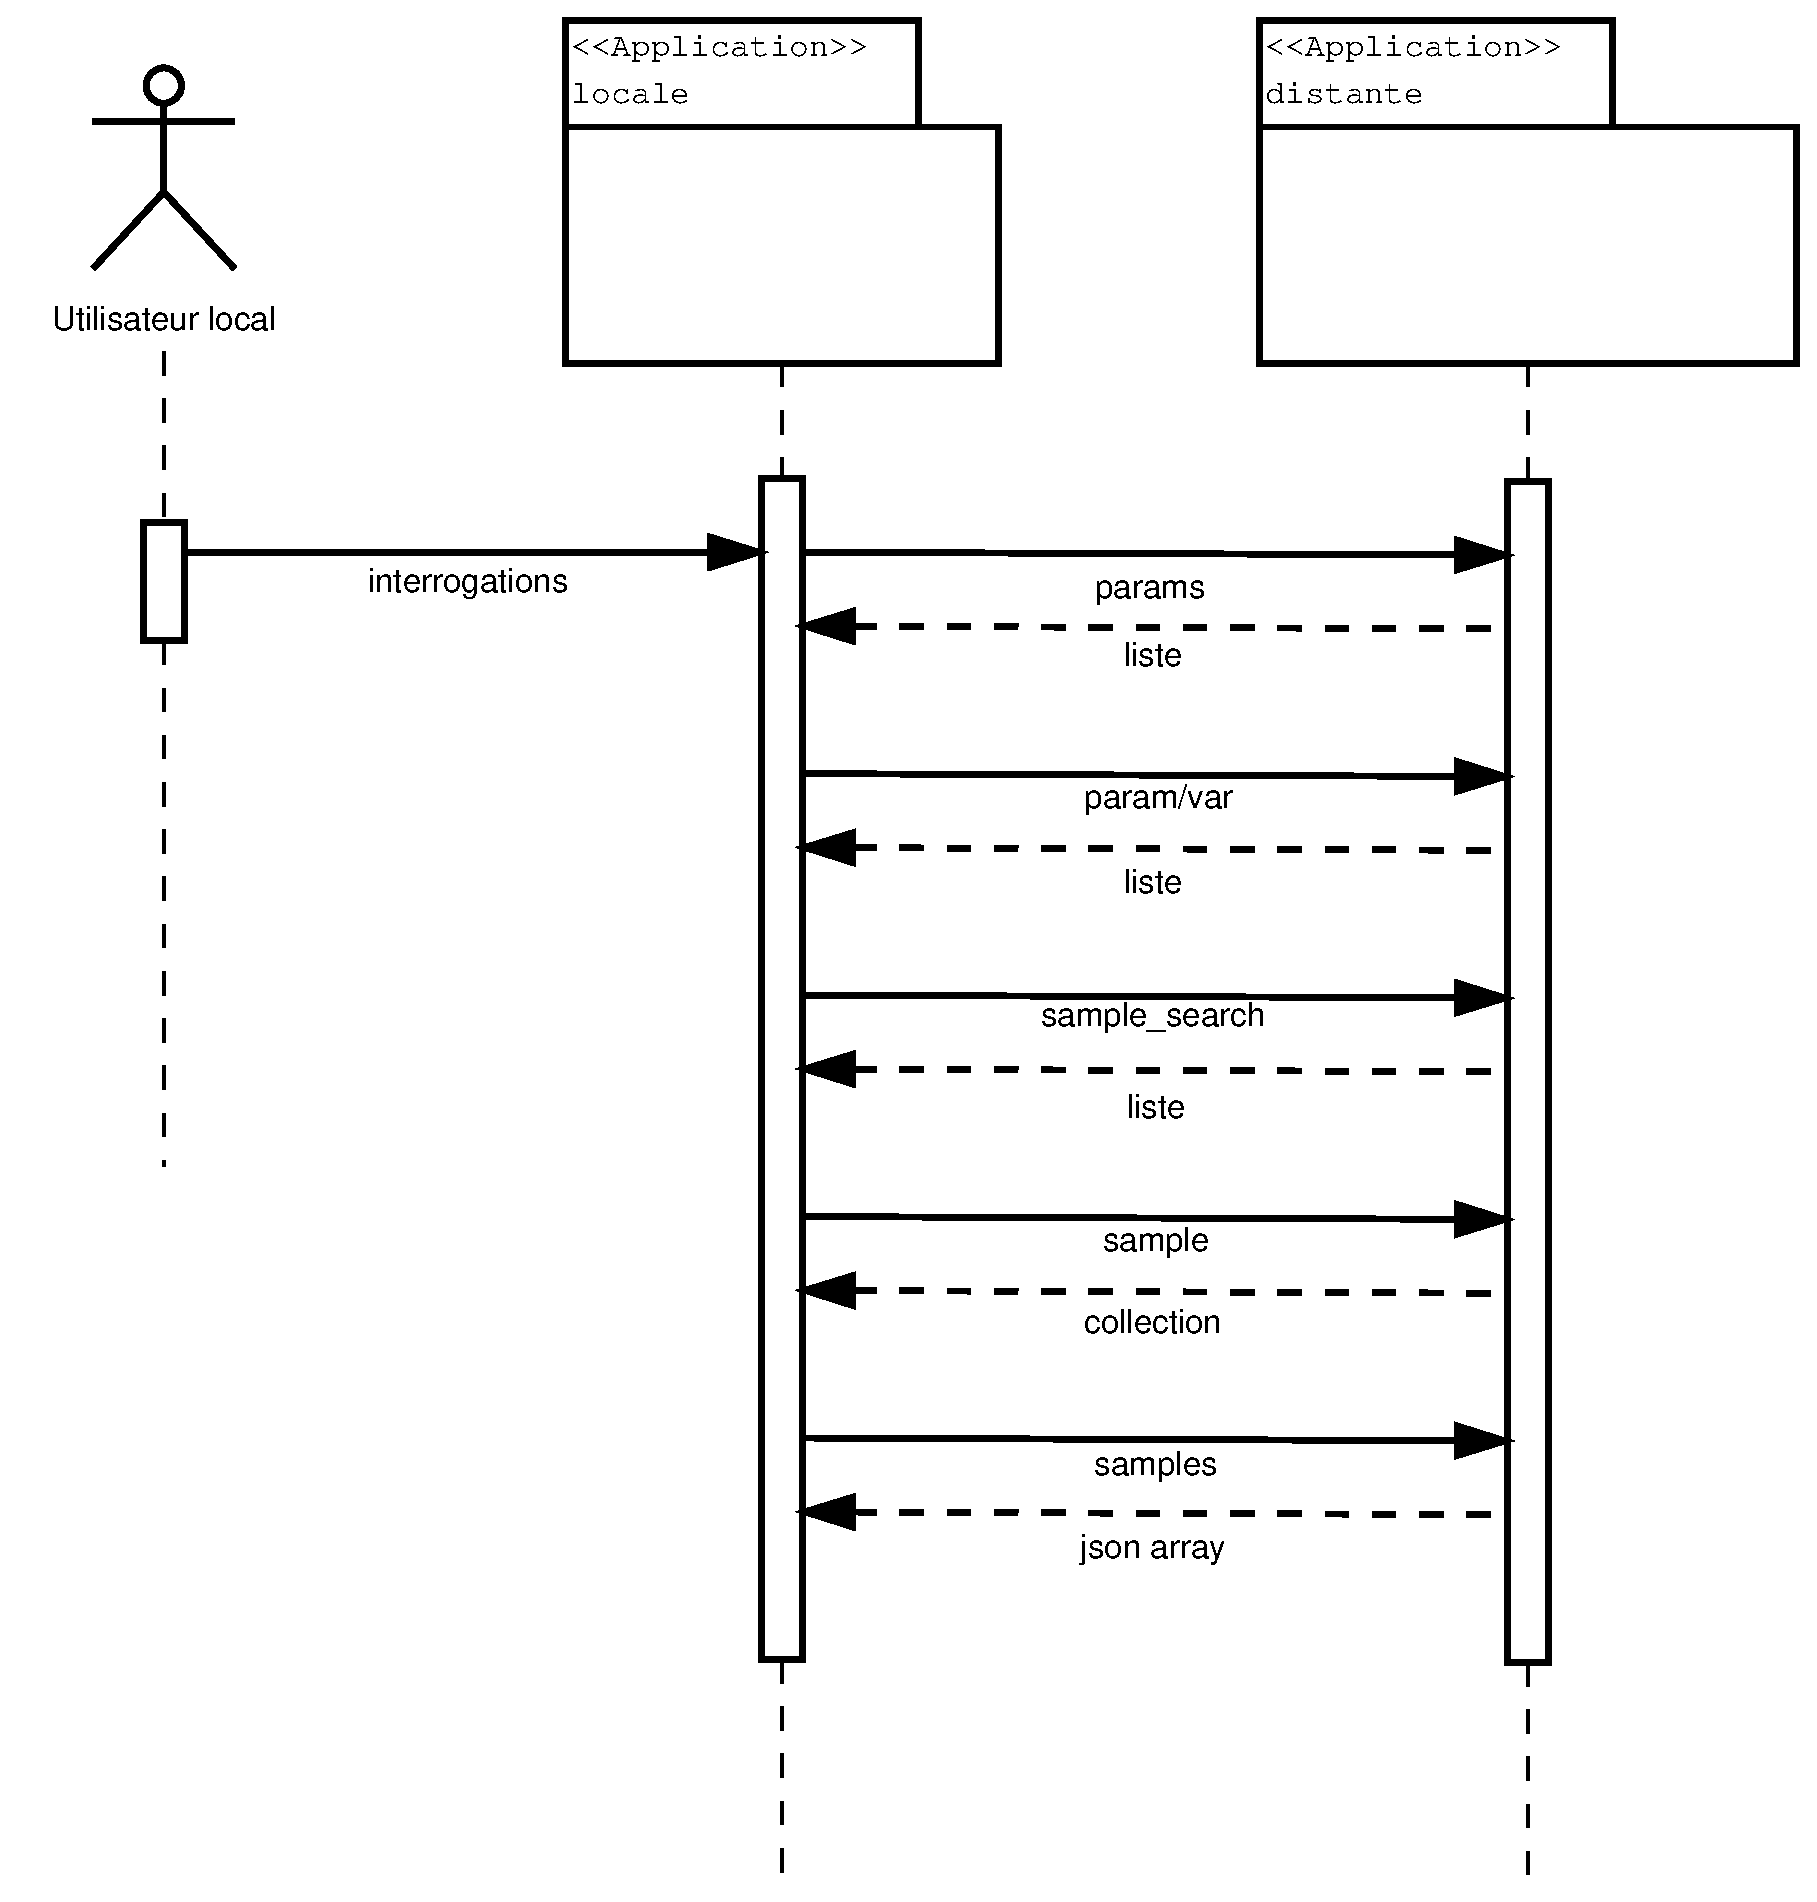
\includegraphics[width=\linewidth]{images/sequence}

Cinq services web ont été identifiés :
\begin{itemize}
\item les deux premiers permettent de récupérer les listes de référence nécessaires pour faire des recherches selon divers paramètres ;
\item le troisième permet de lancer une recherche pour trouver des échantillons ;
\item les deux derniers récupèrent les informations correspondant à un ou plusieurs échantillons respectivement.
\end{itemize}


\subsection{Recherche d'échantillons}
La recherche d'échantillons doit pouvoir s'effectuer selon plusieurs critères :
\begin{itemize}
\item l'identifiant interne (\textit{uid});
\item l'identifiant principal ou des identifiants secondaires;
\item une fourchette de dates de création des échantillons;
\item un type d'échantillons;
\item un projet ou sous-collection;
\item une fourchette d'identifiants internes;
\item un code unique de type GUID ou UUID;
\item le lieu de collecte de l'échantillon;
\item tout autre paramètre traité dans l'application distante.
\end{itemize}

Elle retourne une liste d'échantillons correspondant aux critères indiqués. Le détail des informations retournées est spécifié dans la section \ref{sampleSearch}.

Pour permettre cette recherche, il est nécessaire de récupérer les tables de référence (types d'échantillons, projets ou sous-collections, lieux de collecte...). Les tables utilisables pour la recherche peuvent différer selon les logiciels, et cette liste peut être retrouvée par un service web dédié.

\subsection{Liste des tables de référence}
Ce service permet d'obtenir l'ensemble des tables de référence avec lesquelles il est possible de réaliser une recherche.

\subsection{Contenu des tables de référence}
Ce service récupère le contenu d'une des tables de référence.

\subsection{Récupération des données d'un échantillon}
Ce service permet de récupérer l'ensemble des données concernant un échan\-tillon, y compris les données \og métiers \fg{} si l'utilisateur dispose des droits néces\-saires pour les consulter.

Les données récupérées doivent être suffisamment complètes pour pouvoir être intégrées dans l'application de gestion des échantillons locale.

Elles permettent également une visualisation détaillée de l'échantillon consi\-déré, et contiennent, le cas échéant\footnote{si l'utilisateur dispose des droits adéquats et si l'échantillon dispose de ces informations}, les données \og métiers \fg{} associées.

\subsection{Récupération des données d'une liste d'échantillons}

Il s'agit d'une variante du service web précédent. La liste des échantillons à récupérer est fournie dans une collection Json, soit en utilisant l'UID, soit en utilisant le GUID.

\section{Contraintes liées à la sécurité}

L'accès aux données nécessite une identification préalable de l'utilisateur. Elle est décrite dans le chapitre \ref{oauth}.

\section{Présentation du logiciel Collec}

Collec est un logiciel de gestion de collections d'échantillons, dont l'objectif principal vise à faciliter la recherche d'un échantillon stocké ou de récupérer les informations générales le concernant.

Écrit en PHP, les données sont stockées dans une base de données PostgreSQL. Le logiciel est bâti sur un modèle MVC, tous les accès étant gérés par l'appel à des modules déclarés dans un fichier spécifique. 
Le code de l'application est disponible à l'adresse \url{https://gitlab.com/Irstea/collec}, sous licence AGPL.


La gestion matérielle des échantillons de laboratoire (ou d'expérimentations scientifiques) est une fonctionnalité largement demandée, mais peu couverte jusqu'à présent par les logiciels disponibles, et particulièrement dans le domaine de l'\textit{Open Source}. Collec, dont la première version remonte à l'automne 2016, fait l'objet d'un réel intérêt de la part de la communauté scientifique, ses fonctionnalités et sa facilité d'utilisation le rendant attractif. De nombreux développements complémentaires ont été menés en 2017 pour l'adapter à des cas d'usage non prévus initialement. Ce document vise d'ailleurs à en couvrir certains.

Toutefois, Collec n'est pas conçu comme un système global de gestion de données à la fois techniques -- stockage des échantillons -- et de résultats d'analyse par exemple (pas d'informations métiers complexes\footnote{Dans la pratique, à partir de la version 1.1, il est possible de renseigner quelques informations métiers, mais de manière relativement frustre et sans permettre la complexité des actions envisageables avec des bases de données dédiées.}).
Il n'est pas non plus prévu de mettre en place un hébergement centralisé qui permettrait de gérer tous les échantillons de la sphère de recherche.

\textit{A contrario}, cette organisation permet de créer autant d'instances que néces\-saires, notamment pour gérer des saisies en mode décentralisé (bateau partant en campagne de sondage dans les mers du Sud, collecte d'échantillons depuis des zones non couvertes par Internet, par exemple).

Cette souplesse nécessite de prévoir des mécanismes soit d'interrogation de diverses instances, soit de récupération des informations concernant des échantillons provenant d'autres bases de données. 

